\section*{Zadanie 41.}
\begin{task}

Fala płaska rozchodząca sie w kierunku +0x pada prostopadle na granice w układzie trzech ośrodków:\\
$I \hspace{16} \varepsilon_{1} = \varepsilon_{0} \hspace{30} \mu_{1}=\mu_{0} \hspace{30} \sigma_{1} = 0 $\\
$II \hspace{10} \varepsilon_{2} = 4\varepsilon_{0} \hspace{25} \mu_{2} =\quad ? \hspace{26.5} \sigma_{2} = 0 $\\
$III \ \varepsilon_{3} =\quad ? \hspace{25} \mu_{3}=8\mu_{0} \hspace{25} \sigma_{3} = 0 $\\
gdzie d = 2.5 cm\\
Współczynnik odbicia dla x=0 jest równy 1/3. Wiedząc, że dla pewnej częstotliwości $ f $ grubość ośrodka II stanowi połowę długości fali w tym ośrodku i współczynnik fali stojącej w ośrodku I wynosi jeden wyznaczyć wartości $f, \mu_{2} $ i $ \varepsilon_{3}$. Dla wyznaczonej czestotliwości narysować obwiednię natężenia pola elektrycznego znormalizowaną do amplitudy $E_{30}$ natęzenia pola elektrycznego fali w ośrodku III.\\
\end{task}

\begin{solution}
Współczynnik odbicia dla x=0 jest równy 1/3 (x=0 znajduje się na granicy ośrodków 2 i 3) 
\begin{center}
$\Downarrow $\\
\end{center}
$\Gamma_{2,3} = \frac{Z_{3}-Z_{2}}{Z_{3}+Z{2}} = \frac{1}{3} $\\
$3(Z_{3}-Z_{2}) = Z_{3}+Z_{2}$\\
$3Z_{3}-3Z_{2} = Z_{3}+Z_{2}$\\
$2Z_{3} = 4Z_{2}$\\
$Z_{3} = 2Z_{2}$\\
$\sqrt{\frac{\mu_{3}}{\varepsilon_{3}}} = 2\sqrt{\frac{\mu_{2}}{\varepsilon_{2}}} \quad / ()^{2}$ \\
$\frac{ \mu_{3} }{ \varepsilon_{3} } = 4\frac{\mu_{2}}{\varepsilon_{2}} \qquad \begin{cases} \mu_{3}=8\\\varepsilon_{2}=4\end{cases}$ \\
$ \frac {8}{\varepsilon_{3}} = \not 4 \frac{\mu_{2}}{\not 4} $ \\
$ \mu_{2} = \frac{8}{\varepsilon_{3}}$ \\

dla pewnej częstotliwości f grubość ośrodka II stanowi połowę długości fali w tym ośrodku $\rightarrow$ oznacza to że w ośrodku II mamy do czynienia z tranformatorem półfalowym, czyli takim że $d = \frac{\lambda}{2} \Longleftrightarrow  Z_{1}=Z{3}$\\
z tego wyznaczamy wartość $\varepsilon_{3}$ w nastepujący sposób:\\
$\frac{ \mu_{1} }{ \varepsilon_{1} } = \frac{\mu_{3}}{\varepsilon_{3}}$\\
$1 = \frac{\mu_{3}}{\varepsilon_{3}}$\\
$\varepsilon_{3} = \mu_{3} = 8$\\
$\varepsilon_{3} = 8 \varepsilon_{0} $\\
$\begin{cases} \mu_{2}=1 \quad [\frac{H}{m}]\\\varepsilon_{3}=8 \quad [\frac{F}{m}]\end{cases}$\\
Częstotliwość obliczamy z podstawowego wzoru na częstotliwość fali, tj.
$\lambda = \frac{v}{f} \rightarrow f = \frac{v}{\lambda}$\\
$f = \frac{3 \cdot 10^{8} \frac{m}{s}}{ \sqrt{\mu_{2} \varepsilon_{2}} \cdot 0.05 \ m} = 3 \cdot 10^{9} \ \frac{1}{s} = 3 \cdot 10^{9} \ Hz = 3 \ GHz$\\
\begin{center}
    $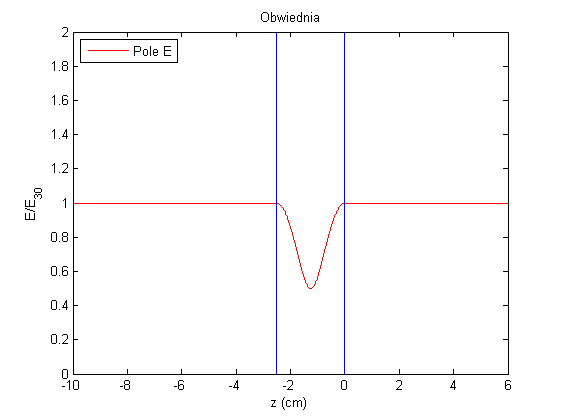
\includegraphics[scale=1]{41}$\\
\end{center}
\end{solution}